%
% File emnlp2018.tex
%
%% Based on the style files for EMNLP 2018, which were
%% Based on the style files for ACL 2018, which were
%% Based on the style files for ACL-2015, with some improvements
%%  taken from the NAACL-2016 style
%% Based on the style files for ACL-2014, which were, in turn,
%% based on ACL-2013, ACL-2012, ACL-2011, ACL-2010, ACL-IJCNLP-2009,
%% EACL-2009, IJCNLP-2008...
%% Based on the style files for EACL 2006 by 
%%e.agirre@ehu.es or Sergi.Balari@uab.es
%% and that of ACL 08 by Joakim Nivre and Noah Smith

\documentclass[11pt,a4paper]{article}
\usepackage[hyperref]{emnlp2018}
\usepackage{times}
\usepackage{latexsym}
\usepackage{graphicx}
\usepackage{url}
\graphicspath{ {images/} }

%\aclfinalcopy % Uncomment this line for the final submission

%\setlength\titlebox{5cm}
% You can expand the titlebox if you need extra space
% to show all the authors. Please do not make the titlebox
% smaller than 5cm (the original size); we will check this
% in the camera-ready version and ask you to change it back.

\newcommand\BibTeX{B{\sc ib}\TeX}
\newcommand\confname{EMNLP 2018}
\newcommand\conforg{SIGDAT}

\title{Bachprop: Using Neural Networks to Solve Composer Classification}

\author{First Author \\
  Affiliation / Address line 1 \\
  Affiliation / Address line 2 \\
  Affiliation / Address line 3 \\
  {\tt email@domain} \\\And
  Second Author \\
  Affiliation / Address line 1 \\
  Affiliation / Address line 2 \\
  Affiliation / Address line 3 \\
  {\tt email@domain} \\}

\date{}

\begin{document}
\maketitle
\begin{abstract}
Music is the ultimate language and shares many common features with the natural language . Both are methods of communication, and have been analyzed in depth and broken down into component parts (grammar for natural languages, rhythms/melodies/harmonies for music). In this paper, we present a state of the art model to classify musical pieces based on their authors. We evaluated our model with the best previous approach and achieved 88\% accuracy compared to their 86\% accuracy on a dataset of 3 composers, Bach, Beethoven, and Haydn. Finally we show that our model can also work with larger set of composers and gain 72\% accuracy on a dataset of 10 composers.
\end{abstract}

\section{Introduction}

It has been more than four decades since Leonard Bernstein called on researchers at his famous lecture at Hardvard University \cite{Bernstein} to create a musical grammar similar to Noam Chomsky's generative grammar \cite{Chomsky}.
Inspired by Bernstein's speech, American linguist Ray Jackendoff and music theorist Fred Lerdahl presented A generative theory of tonal music (GTTM) with the goal of illustrating human's understanding of music. This theory has been influential and inspired further work by other researchers in the field of music cognition which then lead to the creation of musical grammar and inspired other researchers to develop different models for musical grammars. Such models shows that there is a strict hierarchical structure in a musical components. With the advances in technology and computers a new problem has been created and that is to see if computers can also find these strict hierarchical structure in a musical components. In this paper, we developed a model that could identify the composer of a musical piece using these hierarchical structures in a musical component.\\

In this paper, we used NLP techniques to analyze musical passages. A musical piece is broken down into component parts and transform it into a sequence classifier problem and train an LSTM as a sequence classifier. There has been a number of studies on rule based approaches for this problem. Previous works mostly includes producing a generative grammar to capture stylistics features of a musical pieces. However, these studies show that musical style happens in ways musicology and cognitive approaches are still unable to perfectly define them. We believe our approach can cover this flaw and produce better results than those works. \\

One of the challenges of this work is to extract useful musical features for building an accurate classification model. There are number of ways to extract these musical structures and features from a dataset.  In this work, we are looking at high level features extracted from MIDI files; e.g., pitch, duration, tempo, key signature and time signature. MIDI files are symbolic music representations that contain very high level structured information about music. MIDI files describe the start, duration, tempo, volume, and instrument of each note in a musical fragment. The other option would have been to extract information from audio recording of a music which is not the goal of this study.\\ 

In this paper, we are looking at a new approach for building a composer-classification model that can accurately identify the composer of a musical piece. Previous studies on composer recognizer problem were mostly resulted in a binary model that could only recognize if a musical piece was written by a specific composer or not. There has been quite a few studies on a multi-class models but these studies are usually limited to 3 composers.  However, in this paper we introduce a state of the art model to recognize a class of composers with the size of as three times larger than the current state of the art multi class identifier and produces a better accuracy compared to the previous models. The rest of the paper is organized as follows. Section 2 reviews related work. Section 3 explains our approach for building the composer-classification model. Section 4 presents and discuss the measurement results. Section 5 concludes with summary and future work.


\section{Related Works}

With the advances of new techniques in machine learning and deep learning, recognizing a musical piece composer has become the center of attention in the field of music information retrieval (MIR).\\
Buzzanca \cite{Buzz} used a supervised learning approach for musical style recognition of Giovanni Pierluigi da Palestrina. He implemented a neural network that could recognize Pierluigi style with the accuracy of 97\% on the test set. \\
There has been a few studies on style recognition using an n-gram model. Wolkowicz, Kulka, and Keselj \cite{n-gram} used an n-gram model to classify piano files of five composers.  Hillewaere, Manderick, and Conklin \cite{Hillewaere} also used n-gram models to classify musical pieces of two composers (Haydn and Mozart). They achieved the accuracy of 61\%.\\ 
Mearns, Tidhar, and Dixon \cite{Mearns} used a decision tree and naive Bayes models to classify similar musical pieces. The correctly classified 44 out of 66 pieces with seven class ofcomposers. Dor and Reich \cite{Dor} achieved an accuracy of 75\% in classifying keyboard scores between Mozart and Haydn by building a system of decision tree, naive Bayes, support vector machines, and RIPPER classifier. \\
Herremans, Sorensen, and Martens \cite {Herremans} built a four composer-classification models to understand the stylistic differemces between Beethoven, Bach, and Haydn.For the first two models they use an if-then rule set and a decision tree and for the other two models they use a logistic regression model and a support vector machine classifier which produce a more accurate results. They achieved an accuracy of 86\% for the best model. 
In this paper, we present a brand new approach to tackle the composer identifier problem. We use a Long Short Term Memory (LSTM) architecture to produce a composer-classification model to recognize the composer from a musical piece. Our model is a multi-class classifier that can be used to identify the composer of a musical piece. 


\section{Approach}
To solve this problem, we are taking a neural network based approach to multiclass classification. We divide the dataset into training, validation, and test datasets, with an $80:10:10$ split. The first step is to preprocess the MIDI file into a sequence of feature vectors. We subdivide the MIDI file into 32nd note divisions in time, and for each division we compute a set of features. The most important feature is what notes are being played at that division of time; this corresponds to the time between the \texttt{note\_on}  and \texttt{note\_off}  messages in the file. At this stage, we also transpose the notes into the key of C or C minor based on the currently active key signature. This helps normalize the data and remove any noise caused by key selection. We then convert the set of notes being played into a one-hot vector. We also extract the tempo, time signature, and key signature from each division of time and concatenate those features to the note feature (tempo being treated as continuous, while time and key are treated as categorical one-hot vectors). We then take each continuous  segment of 64 divisions (2 measures of music in 4/4 time) as one training example.\\
The input sequence is then passed into an LSTM layer. We found that using a 150 length hidden state vector achieved the best results over our validation dataset. Our architecture allows users to set various parameters such as number if hidden layers, sequence length, batch size, and learning rate. The final output of the LSTM layer is then passed into a fully connected linear layer, and finally into a softmax layer to compute the probabilities for each composer. We then pick the composer with the highest probability as the final result. For more accurate results, we take the prediction from multiple musical samples of the same composer and take the majority, i.e. if we look at 32 beats, we try to predict every 8 beat, grouping the results and take the majority as our final prediction. For better clarification, we use the term piece accuracy for computing the accuracy of this method.\\
To train the network, we are using mini-batches of size 500 and the Adam optimizer with a decaying learning rate. Since our dataset is highly imbalanced (we have several times more examples from Beethoven/Bach than lesser known composers), we oversample the composers with fewer unique examples to compensate. The optimizer is set to minimize the cross entropy over the training dataset. The loss corresponds to the cross entropy error of our prediction compared to the actual composer of the musical piece. Our deep learning implementation was done in TensorFlow.\\

\section{Experiments}

\subsection{Data}
In this paper we use the KernScores database which contains musical pieces as a MIDI files. The KernScores database is a large collection of virtual musical scores made available by the Center for Computer Assisted Research in the humanities at Stanford University (CCARH). The KernScores database has a total of $7866496$ notes and is available online at  kern.ccarh.org.
For the baseline, we are comparing our results with the Herremans, Sorensen, and Martens \cite {Herremans} results. They also used the same database for running their experiments. Since they selected Bach, Beethoven, and Haydn for inclusion in their classification models, we also use these composers in our experimental results. An overview of the selected composers was given in table 1.

\begin{table}[t!]
\begin{center}
\begin{tabular}{|l|l|}
\hline \bf Composers & \bf Examples \\ \hline
Beethoven & 10526 \\
Haydn & 9758 \\
Bach & 8544\\
Corelli & 3555\\
Buxtehude & 3728\\
Monteverdi & 302 \\
Foster & 350\\
Frescobaldi & 1904\\
Josquin & 79\\
Schumann & 82\\
Joplin & 1788\\
Gershwin & 890\\
Giovannelli & 9758\\
Mozart & 6733  \\
\hline
\end{tabular}
\end{center}
\caption{\label{composer-table}List of composers. }
\end{table}

\subsection{Baseline}
For our baseline, we had results of  Herremans, Sorensen, and Martens \cite {Herremans} classifier on three composers Beethoven, Bach, and Haydn. Our model out perform their best model. In table 2, we are comparing our model with three diffrent models that they used in their paper. Since they use the whole musical piece to classify, we compare their accuracy with our piece accuracy. Mozart in this set of composers has the least accuracy (47\%). We believe this is because his work covered a large variety of things which makes it difficult for our model to be identified.

\begin{table}[t!]
\begin{center}
\begin{tabular}{|l|l|}
\hline \bf Method & \bf Accuracy (\%) \\ \hline
\underline{LSTM} & 87.3 \\
Support vector machines & 86 \\
Logistic regression & 83\\
C4.5 decision tree & 79\\
RIPPER rule set & 77\\
\hline
\end{tabular}
\end{center}
\caption{\label{resutls-table} Model Evaluation. }
\end{table}

\subsection{Generalized classifier}
Unfortunately all the previous works only considered up to 3 composers in their classifier but we were able to generalize our approach and get good accuracy for more complex datasets. We were able to get the accuracy of 72\% on our test set using the same architecture as in the baseline experiment. Table 3 shows the accuracy for each composers. 
\begin{table}[t!]
\begin{center}
\begin{tabular}{|l|l|}
\hline \bf Composers & \bf Accuracy (\%)\\ \hline
Beethoven & 72 \\
Mozart & 47\\
Foster & 59\\
Frescobaldi & 99\\
Josquin & 65\\
Schumann & 62\\
Joplin & 93\\
Gershwin & 95\\
Giovannelli & 96\\
Vivaldi & 95  \\
\hline
\end{tabular}
\end{center}
\caption{\label{test-accuracy-table}Accuracy. }
\end{table}

\begin{figure}[h]
\caption{Piece Accuracy}
\centering
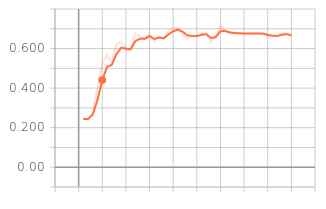
\includegraphics[width=0.5\textwidth]{Gaccuracy.png}
\end{figure}

\begin{figure}[h]
\caption{Validation Accuracy}
\centering
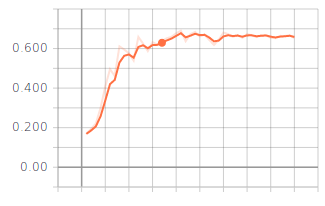
\includegraphics[width=0.5\textwidth]{vaccuracy.png}
\end{figure}


\subsection{Conclusion and Future Work}


\label{sect:pdf}

For the production of the electronic manuscript you must use Adobe's
Portable Document Format (PDF). PDF files are usually produced from
\LaTeX\ using the \textit{pdflatex} command. If your version of
\LaTeX\ produces Postscript files, you can convert these into PDF
using \textit{ps2pdf} or \textit{dvipdf}. On Windows, you can also use
Adobe Distiller to generate PDF.

Please make sure that your PDF file includes all the necessary fonts
(especially tree diagrams, symbols, and fonts with Asian
characters). When you print or create the PDF file, there is usually
an option in your printer setup to include none, all or just
non-standard fonts.  Please make sure that you select the option of
including ALL the fonts. \textbf{Before sending it, test your PDF by
  printing it from a computer different from the one where it was
  created.} Moreover, some word processors may generate very large PDF
files, where each page is rendered as an image. Such images may
reproduce poorly. In this case, try alternative ways to obtain the
PDF. One way on some systems is to install a driver for a postscript
printer, send your document to the printer specifying ``Output to a
file'', then convert the file to PDF.

It is of utmost importance to specify the \textbf{A4 format} (21 cm
x 29.7 cm) when formatting the paper. When working with
{\tt dvips}, for instance, one should specify {\tt -t a4}.
Or using the command \verb|\special{papersize=210mm,297mm}| in the latex
preamble (directly below the \verb|\usepackage| commands). Then using 
{\tt dvipdf} and/or {\tt pdflatex} which would make it easier for some.

Print-outs of the PDF file on A4 paper should be identical to the
hardcopy version. If you cannot meet the above requirements about the
production of your electronic submission, please contact the
publication chairs as soon as possible.

\subsection{Layout}
\label{ssec:layout}

Format manuscripts two columns to a page, in the manner these
instructions are formatted. The exact dimensions for a page on A4
paper are:

\begin{itemize}
\item Left and right margins: 2.5 cm
\item Top margin: 2.5 cm
\item Bottom margin: 2.5 cm
\item Column width: 7.7 cm
\item Column height: 24.7 cm
\item Gap between columns: 0.6 cm
\end{itemize}

\noindent Papers should not be submitted on any other paper size.
 If you cannot meet the above requirements about the production of 
 your electronic submission, please contact the publication chairs 
 above as soon as possible.

\subsection{Fonts}

For reasons of uniformity, Adobe's {\bf Times Roman} font should be
used. In \LaTeX2e{} this is accomplished by putting

\begin{quote}
\begin{verbatim}
\usepackage{times}
\usepackage{latexsym}
\end{verbatim}
\end{quote}
in the preamble. If Times Roman is unavailable, use {\bf Computer
  Modern Roman} (\LaTeX2e{}'s default).  Note that the latter is about
  10\% less dense than Adobe's Times Roman font.

\begin{table}[t!]
\begin{center}
\begin{tabular}{|l|rl|}
\hline \bf Type of Text & \bf Font Size & \bf Style \\ \hline
paper title & 15 pt & bold \\
author names & 12 pt & bold \\
author affiliation & 12 pt & \\
the word ``Abstract'' & 12 pt & bold \\
section titles & 12 pt & bold \\
document text & 11 pt  &\\
captions & 10 pt & \\
abstract text & 10 pt & \\
bibliography & 10 pt & \\
footnotes & 9 pt & \\
\hline
\end{tabular}
\end{center}
\caption{\label{font-table} Font guide. }
\end{table}

\subsection{The First Page}
\label{ssec:first}

Center the title, author's name(s) and affiliation(s) across both
columns. Do not use footnotes for affiliations. Do not include the
paper ID number assigned during the submission process. Use the
two-column format only when you begin the abstract.

{\bf Title}: Place the title centered at the top of the first page, in
a 15-point bold font. (For a complete guide to font sizes and styles,
see Table~\ref{font-table}) Long titles should be typed on two lines
without a blank line intervening. Approximately, put the title at 2.5
cm from the top of the page, followed by a blank line, then the
author's names(s), and the affiliation on the following line. Do not
use only initials for given names (middle initials are allowed). Do
not format surnames in all capitals ({\em e.g.}, use ``Mitchell'' not
``MITCHELL'').  Do not format title and section headings in all
capitals as well except for proper names (such as ``BLEU'') that are
conventionally in all capitals.  The affiliation should contain the
author's complete address, and if possible, an electronic mail
address. Start the body of the first page 7.5 cm from the top of the
page.

The title, author names and addresses should be completely identical
to those entered to the electronical paper submission website in order
to maintain the consistency of author information among all
publications of the conference. If they are different, the publication
chairs may resolve the difference without consulting with you; so it
is in your own interest to double-check that the information is
consistent.

{\bf Abstract}: Type the abstract at the beginning of the first
column. The width of the abstract text should be smaller than the
width of the columns for the text in the body of the paper by about
0.6 cm on each side. Center the word {\bf Abstract} in a 12 point bold
font above the body of the abstract. The abstract should be a concise
summary of the general thesis and conclusions of the paper. It should
be no longer than 200 words. The abstract text should be in 10 point font.

{\bf Text}: Begin typing the main body of the text immediately after
the abstract, observing the two-column format as shown in 


the present document. Do not include page numbers.

{\bf Indent}: Indent when starting a new paragraph, about 0.4 cm. Use 11 points for text and subsection headings, 12 points for section headings and 15 points for the title. 


\begin{table}
\centering
\small
\begin{tabular}{cc}
\begin{tabular}{|l|l|}
\hline
{\bf Command} & {\bf Output}\\\hline
\verb|{\"a}| & {\"a} \\
\verb|{\^e}| & {\^e} \\
\verb|{\`i}| & {\`i} \\ 
\verb|{\.I}| & {\.I} \\ 
\verb|{\o}| & {\o} \\
\verb|{\'u}| & {\'u}  \\ 
\verb|{\aa}| & {\aa}  \\\hline
\end{tabular} & 
\begin{tabular}{|l|l|}
\hline
{\bf Command} & {\bf  Output}\\\hline
\verb|{\c c}| & {\c c} \\ 
\verb|{\u g}| & {\u g} \\ 
\verb|{\l}| & {\l} \\ 
\verb|{\~n}| & {\~n} \\ 
\verb|{\H o}| & {\H o} \\ 
\verb|{\v r}| & {\v r} \\ 
\verb|{\ss}| & {\ss} \\\hline
\end{tabular}
\end{tabular}
\caption{Example commands for accented characters, to be used in, {\em e.g.}, \BibTeX\ names.}\label{tab:accents}
\end{table}

\subsection{Sections}

{\bf Headings}: Type and label section and subsection headings in the
style shown on the present document.  Use numbered sections (Arabic
numerals) in order to facilitate cross references. Number subsections
with the section number and the subsection number separated by a dot,
in Arabic numerals.
Do not number subsubsections.

\begin{table*}[t!]
\centering
\begin{tabular}{lll}
  output & natbib & previous \conforg{} style files\\
  \hline
  \citep{Gusfield:97} & \verb|\citep| & \verb|\cite| \\
  \citet{Gusfield:97} & \verb|\citet| & \verb|\newcite| \\
  \citeyearpar{Gusfield:97} & \verb|\citeyearpar| & \verb|\shortcite| \\
\end{tabular}
\caption{Citation commands supported by the style file.
  The citation style is based on the natbib package and
  supports all natbib citation commands.
  It also supports commands defined in previous \conforg{} style files
  for compatibility.
  }
\end{table*}

{\bf Citations}: Citations within the text appear in parentheses
as~\cite{Gusfield:97} or, if the author's name appears in the text
itself, as Gusfield~\shortcite{Gusfield:97}.
Using the provided \LaTeX\ style, the former is accomplished using
{\small\verb|\cite|} and the latter with {\small\verb|\shortcite|} or {\small\verb|\newcite|}. Collapse multiple citations as in~\cite{Gusfield:97,Aho:72}; this is accomplished with the provided style using commas within the {\small\verb|\cite|} command, {\em e.g.}, {\small\verb|\cite{Gusfield:97,Aho:72}|}. Append lowercase letters to the year in cases of ambiguities.  
 Treat double authors as
in~\cite{Aho:72}, but write as in~\cite{Chandra:81} when more than two
authors are involved. Collapse multiple citations as
in~\cite{Gusfield:97,Aho:72}. Also refrain from using full citations
as sentence constituents.

We suggest that instead of
\begin{quote}
  ``\cite{Gusfield:97} showed that ...''
\end{quote}
you use
\begin{quote}
``Gusfield \shortcite{Gusfield:97}   showed that ...''
\end{quote}

If you are using the provided \LaTeX{} and Bib\TeX{} style files, you
can use the command \verb|\citet| (cite in text)
to get ``author (year)'' citations.

If the Bib\TeX{} file contains DOI fields, the paper
title in the references section will appear as a hyperlink
to the DOI, using the hyperref \LaTeX{} package.
To disable the hyperref package, load the style file
with the \verb|nohyperref| option: \\{\small
\verb|\usepackage[nohyperref]{acl2018}|}


\textbf{Digital Object Identifiers}: As part of our work to make ACL
materials more widely used and cited outside of our discipline, ACL
has registered as a CrossRef member, as a registrant of Digital Object
Identifiers (DOIs), the standard for registering permanent URNs for
referencing scholarly materials. \conforg{} has \textbf{not} adopted the
ACL policy of requiring camera-ready references to contain the appropriate
  DOIs (or as a second resort, the hyperlinked ACL Anthology
  Identifier). But we certainly encourage you to use
  Bib\TeX\ records that contain DOI or URLs for any of the ACL
  materials that you reference. Appropriate records should be found
for most materials in the current ACL Anthology at
\url{http://aclanthology.info/}.

As examples, we cite \cite{P16-1001} to show you how papers with a DOI
will appear in the bibliography.  We cite \cite{C14-1001} to show how
papers without a DOI but with an ACL Anthology Identifier will appear
in the bibliography.  

\textbf{Anonymity:} As reviewing will be double-blind, the submitted
version of the papers should not include the authors' names and
affiliations. Furthermore, self-references that reveal the author's
identity, {\em e.g.},
\begin{quote}
``We previously showed \cite{Gusfield:97} ...''  
\end{quote}
should be avoided. Instead, use citations such as 
\begin{quote}
``\citeauthor{Gusfield:97} \shortcite{Gusfield:97}
previously showed ... ''
\end{quote}

Preprint servers such as arXiv.org and workshops that do not
have published proceedings are not considered archival for purposes of
submission. However, to preserve the spirit of blind review, authors
are encouraged to refrain from posting until the completion of the
review process. Otherwise, authors must state in the online submission
form the name of the workshop or preprint server and title of the
non-archival version. The submitted version should be suitably
anonymized and not contain references to the prior non-archival
version. Reviewers will be told: ``The author(s) have notified us that
there exists a non-archival previous version of this paper with
significantly overlapping text. We have approved submission under
these circumstances, but to preserve the spirit of blind review, the
current submission does not reference the non-archival version.''

\textbf{Please do not use anonymous citations} and do not include
 when submitting your papers. Papers that do not
conform to these requirements may be rejected without review.

\textbf{References}: Gather the full set of references together under
the heading {\bf References}; place the section before any Appendices,
unless they contain references. Arrange the references alphabetically
by first author, rather than by order of occurrence in the text.
By using a .bib file, as in this template, this will be automatically 
handled for you. See the \verb|\bibliography| commands near the end for more.

Provide as complete a citation as possible, using a consistent format,
such as the one for {\em Computational Linguistics\/} or the one in the 
{\em Publication Manual of the American 
Psychological Association\/}~\cite{APA:83}. Use of full names for
authors rather than initials is preferred. A list of abbreviations
for common computer science journals can be found in the ACM 
{\em Computing Reviews\/}~\cite{ACM:83}.

The \LaTeX{} and Bib\TeX{} style files provided roughly fit the
American Psychological Association format, allowing regular citations, 
short citations and multiple citations as described above.  

\begin{itemize}
\item Example citing an arxiv paper: \cite{rasooli-tetrault-2015}. 
\item Example article in journal citation: \cite{Ando2005}.
\item Example article in proceedings, with location: \cite{borsch2011}.
\item Example article in proceedings, without location: \cite{andrew2007scalable}.
\end{itemize}
See corresponding .bib file for further details.

Submissions should accurately reference prior and related work, including code and data. If a piece of prior work appeared in multiple venues, the version that appeared in a refereed, archival venue should be referenced. If multiple versions of a piece of prior work exist, the one used by the authors should be referenced. Authors should not rely on automated citation indices to provide accurate references for prior and related work.

{\bf Appendices}: Appendices, if any, directly follow the text and the
references (but see above).  Letter them in sequence and provide an
informative title: {\bf Appendix A. Title of Appendix}.

\subsection{URLs}

URLs can be typeset using the \verb|\url| command. However, very long
URLs cause a known issue in which the URL highlighting may incorrectly
cross pages or columns in the document. Please check carefully for
URLs too long to appear in the column, which we recommend you break,
shorten or place in footnotes. Be aware that actual URL should appear
in the text in human-readable format; neither internal nor external
hyperlinks will appear in the proceedings.

\subsection{Footnotes}

{\bf Footnotes}: Put footnotes at the bottom of the page and use 9
point font. They may be numbered or referred to by asterisks or other
symbols.\footnote{This is how a footnote should appear.} Footnotes
should be separated from the text by a line.\footnote{Note the line
separating the footnotes from the text.}

\subsection{Graphics}

{\bf Illustrations}: Place figures, tables, and photographs in the
paper near where they are first discussed, rather than at the end, if
possible.  Wide illustrations may run across both columns.  Color
illustrations are discouraged, unless you have verified that  
they will be understandable when printed in black ink.

{\bf Captions}: Provide a caption for every illustration; number each one
sequentially in the form:  ``Figure 1. Caption of the Figure.'' ``Table 1.
Caption of the Table.''  Type the captions of the figures and 
tables below the body, using 11 point text.


\subsection{Accessibility}
\label{ssec:accessibility}

In an effort to accommodate people who are color-blind (as well as those printing
to paper), grayscale readability for all accepted papers will be
encouraged.  Color is not forbidden, but authors should ensure that
tables and figures do not rely solely on color to convey critical
distinctions. A simple criterion: All curves and points in your figures should be clearly distinguishable without color.

% Min: no longer used as of ACL 2018, following ACL exec's decision to
% remove this extra workflow that was not executed much.
% BEGIN: remove
%% \section{XML conversion and supported \LaTeX\ packages}

%% Following ACL 2014 we will also we will attempt to automatically convert 
%% your \LaTeX\ source files to publish papers in machine-readable 
%% XML with semantic markup in the ACL Anthology, in addition to the 
%% traditional PDF format.  This will allow us to create, over the next 
%% few years, a growing corpus of scientific text for our own future research, 
%% and picks up on recent initiatives on converting ACL papers from earlier 
%% years to XML. 

%% We encourage you to submit a ZIP file of your \LaTeX\ sources along
%% with the camera-ready version of your paper. We will then convert them
%% to XML automatically, using the LaTeXML tool
%% (\url{http://dlmf.nist.gov/LaTeXML}). LaTeXML has \emph{bindings} for
%% a number of \LaTeX\ packages, including the ACL 2018 stylefile. These
%% bindings allow LaTeXML to render the commands from these packages
%% correctly in XML. For best results, we encourage you to use the
%% packages that are officially supported by LaTeXML, listed at
%% \url{http://dlmf.nist.gov/LaTeXML/manual/included.bindings}
% END: remove

\section{Translation of non-English Terms}

It is also advised to supplement non-English characters and terms
with appropriate transliterations and/or translations
since not all readers understand all such characters and terms.
Inline transliteration or translation can be represented in
the order of: original-form transliteration ``translation''.

\section{Length of Submission}
\label{sec:length}

The \confname{} main conference accepts submissions of long papers and
short papers.
 Long papers may consist of up to eight (8) pages of
content plus unlimited pages for references. Upon acceptance, final
versions of long papers will be given one additional page -- up to nine (9)
pages of content plus unlimited pages for references -- so that reviewers' comments
can be taken into account. Short papers may consist of up to four (4)
pages of content, plus unlimited pages for references. Upon
acceptance, short papers will be given five (5) pages in the
proceedings and unlimited pages for references. 

For both long and short papers, all illustrations and tables that are part
of the main text must be accommodated within these page limits, observing
the formatting instructions given in the present document. Supplementary
material in the form of appendices does not count towards the page limit; see appendix A for further information.

However, note that supplementary material should be supplementary
(rather than central) to the paper, and that reviewers may ignore
supplementary material when reviewing the paper (see Appendix
\ref{sec:supplemental}). Papers that do not conform to the specified
length and formatting requirements are subject to be rejected without
review.

Workshop chairs may have different rules for allowed length and
whether supplemental material is welcome. As always, the respective
call for papers is the authoritative source.

\section*{Acknowledgments}

The acknowledgments should go immediately before the references.  Do
not number the acknowledgments section. Do not include this section
when submitting your paper for review. \\

\noindent {\bf Preparing References:} \\

Include your own bib file like this:
{\small\verb|\bibliographystyle{acl_natbib_nourl}|
\verb|\bibliography{emnlp2018}|}

Where \verb|emnlp2018| corresponds to the {\tt emnlp2018.bib} file.
\bibliography{emnlp2018}
\bibliographystyle{acl_natbib_nourl}

\appendix

\section{Supplemental Material}
\label{sec:supplemental}
Each \confname{} submission can be accompanied by a single PDF
appendix, one {\small\tt.tgz} or {\small\tt.zip} appendix containing
software, and one {\small\tt.tgz} or {\small\tt.zip} appendix
containing data.

Submissions may include resources (software and/or data) used in in
the work and described in the paper. Papers that are submitted with
accompanying software and/or data may receive additional credit toward
the overall evaluation score, and the potential impact of the software
and data will be taken into account when making the
acceptance/rejection decisions. Any accompanying software and/or data
should include licenses and documentation of research review as
appropriate.

\confname{} also encourages the submission of supplementary material
to report preprocessing decisions, model parameters, and other details
necessary for the replication of the experiments reported in the
paper. Seemingly small preprocessing decisions can sometimes make a
large difference in performance, so it is crucial to record such
decisions to precisely characterize state-of-the-art methods.

Nonetheless, supplementary material should be supplementary (rather
than central) to the paper. {\bf Submissions that misuse the supplementary 
material may be rejected without review.}
Essentially, supplementary material may include explanations or details
of proofs or derivations that do not fit into the paper, lists of
features or feature templates, sample inputs and outputs for a system,
pseudo-code or source code, and data. (Source code and data should
be separate uploads, rather than part of the paper).

The paper should not rely on the supplementary material: while the paper
may refer to and cite the supplementary material and the supplementary material will be available to the
reviewers, they will not be asked to review the
supplementary material.

Appendices ({\em i.e.} supplementary material in the form of proofs, tables,
or pseudo-code) should be {\bf uploaded as supplementary material} when submitting the paper for review.
Upon acceptance, the appendices come after the references, as shown here. Use
\verb|\appendix| before any appendix section to switch the section
numbering over to letters.

\end{document}
